\chapter{Architectuur van het ontworpen systeem}

Alle onderdelen van het ontworpen systeem zijn onderling onafhankelijk van elkaar. Dit maakt een robuuste, gedistribueerde eenheid waaraan relatief eenvoudig nieuwe componenten kunnen worden toegevoegd. De flow van het programma wordt gecontroleerd door de \textit{FlowController}. Deze zal de flow van het programma bijhouden en alle interactie met de gebruiker verzorgen. 
\textbf{TODO: Meer over de flow en de controller volgt in hoofdstuk \ref{flowcontroller}.}

\textbf{TODO: Wat mogen we verwachten in dit hoofdstuk? Geef overzicht}


\section{TODO: Verwerken van documenten} 
\subsection{\textit{Preprocessing} van tekstdocumenten}\label{bag-of-words}
Om alle woorden te verkrijgen die gebruikt worden in een bepaalde tekst, wordt een \textit{tokenization}\label{tokenization} proces toegepast. Dit zorgt ervoor dat een tekstdocument gesplitst wordt in een stroom van woorden door alle leestekens te verwijderen en alle tabs en niet-tekstuele karakters door spaties te vervangen. De set van verschillende woorden uit alle tekstdocumenten wordt samengevoegd tot het woordenboek van de documentencollectie. 

Het is echter ook mogelijk om een N-Gram tokenizer \cite{McNamee2004} te gebruiken. Deze geeft de mogelijkheid om eventueel twee of drie woorden samen te nemen en die als \'e\'en woord in onze documentencollectie te zien. Dit kan voordeel geven bij o.a. personennamen, welke vaak bestaan uit twee woorden die voor een tekst belangrijk zouden kunnen zijn. Uiteraard wordt een eigennaam ook opgepikt indien alle woorden apart beschouwd worden.

Om de grootte van het woordenboek en dus de dimensionaliteit van de beschrijving van de documentencollectie te verkleinen, wordt de set van woorden verder gereduceerd door het toepassen van filters of \textit{stemming}salgoritmes. 

Filters verwijderen woorden van het woordenboek en dus uit de documenten. De filtering die het meest wordt toegepast op tekstuele collecties is stopwoordfiltering. De stopwoorden die verwijderd worden zijn woorden die weinig of geen inhoud hebben. Voorbeelden zijn lidwoorden, verbindingswoorden, voorzetsels, etc. \\
Stemmingsalgoritmes proberen een woord om te vormen tot de standaardvorm van dat woord. Dit doen ze bijvoorbeeld door meervouden van zelfstandige naamwoorden naar het enkelvoud om te zetten of door werkwoorden naar hun stam te vereenvoudigen. Het stemmingalgoritme dat hier gebruikt wordt is Porters stemming algoritme voor de Nederlandse taal \cite{Kraaij1994}. Het is een implementatie van Porters stemming algoritme \cite{Porter1980}, dat origineel enkel voor de Engelse taal werd ontworpen.

\subsection{Vector space model}\label{vector-space-model}
Ondanks de simpele datastructuur zorgt het vector space model ervoor dat grote collecties documenten effici\"ent kunnen geanalyseerd worden. Het representeert documenten als vectors in een $m$-dimensionale ruimte. Elk document $d$ uit de documentencollectie is beschreven als een numerieke\textit{ feature vector} $w(d) = (x(d,t_1),...,x(d,t_m))$ waarbij $T=\{t_1,...,t_m\}$ het woordenboek voorstelt. De hoofdtaak van de vector space representatie van documenten is het vinden van een geschikte encodering van de feature vector. 

Elk element van de vector representeert meestal een woord (of groep van woorden) van de documentencollectie. De simpelste manier om een document te encoderen is om \textit{binary term} vectoren te gebruiken. Als een woord voorkomt in het document wordt het corresponderende element op \'e\'en gezet, komt het niet voor dan is het nul. De encodering wordt zo herleid tot een simpele Booleaanse vergelijking. Hierbij wordt de belangrijkheid van elk woord als gelijkwaardig beschouwd. 

Om de performantie te verbeteren kunnen \textit{term weighting schemes} worden gebruikt \cite{Salton1988}. Het gewicht dat toegekend wordt aan een woord reflecteert de belangrijkheid of relevantie van dat woord in een specifiek document of collectie. Een woord met hoge frequentie in bepaalde documenten, maar dat weinig of niet voorkomt in de volledige documentencollectie wordt een groot gewicht toebedeeld. Een gewicht $w(d,t)$ voor term $t$ in document $d$ wordt berekend als de term frequency $tf(d,t)$ vermenigvuldigd met de inverse document frequency $idf(t)$ - gedefinieerd als $idf(t)=\log{\frac{N}{n_t}})$. Dit beschrijft de specifiteit van een bepaalde term in een documentencollectie. 

Naast term frequency en inverse document frequency wordt een normalisatie toegepast om ervoor te zorgen dat alle documenten dezelfde kans hebben om gevonden te worden, onafhankelijk van hun lengte. Deze techniek heeft zijn nut reeds bewezen in de praktijk . 
\begin{equation}\label{eq:tfidf}
w(d,t) = \frac{tf(dt)\log{\frac{N}{N_t}}}{\sqrt{\sum_{j=1}^{m}tf(d,t_j)^2(log(\frac{N}{n_{t_j}}))^2}}
\end{equation}
Hierbij stelt $N$ de grootte van de documentencollectie $D$ voor en is $n_t$ het aantal documenten in $D$ dat term $t$ bevat.

\subsection{Feature selection}
Feature selection of attribute selection zorgt ervoor dat attributen die niet relevant zijn verwijderd worden. Dit zorgt er o.a. voor dat de dataset kleiner wordt, waardoor minder rekenkracht en zoekruimte vereist is bij de effectieve verwerking van het vector model. Volgens \cite{Liu2005} is het \'e\'en van de meest belangrijke en meest gebruikte technieken voor data preprocessing bij data mining. Het reduceert het aantal features, het verwijdert irrelevante of redundante data en het zorgt er bijgevolg voor dat data mining algoritmes sneller werken. Het zorgt er o.m. ook voor dat de voorspelde accuraatheid en begrijpbaarheid van de resultaten verbeterd wordt. Feature selection is vooral interessant bij text mining, omdat er een hoge dimensionaliteit is van de features en er veel irrelevante features voorkomen.

Als de dimensionaliteit van een domein bovendien vergroot wordt, verhoogt het aantal features $N$. Een optimale subset van features vinden is zeer moeilijk en veel problemen gerelateerd aan feature selection zijn NP-moeilijk. Volgens \cite{Liu2005} bestaat een typisch feature selection proces uit vier stappen (zie figuur \ref{fig:feature-selection}); subset generatie, subset evaluatie, stopcriterium en resultatenvalidatie.

\begin{figure}[h]
	\caption{Vier stappen in feature selection}
	\label{fig:feature-selection}
	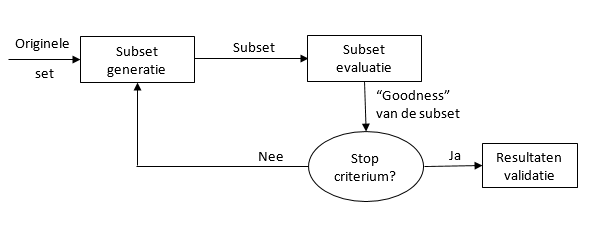
\includegraphics[width=\textwidth]{fig/feature-selection}
\end{figure}

Subset generatie is een zoekprocedure die kandidaat feature subsets produceert voor evaluatie met een bepaalde zoekstrategie. Elke kandidaat subset wordt ge\"evalueerd en vergeleken met de vorige beste volgens een bepaald criterium. Als de nieuwe subset beter is, wordt de vorige beste subset vervangen. Dit proces wordt herhaald tot een bepaald stopcriterium is bereikt. Dan wordt de geselecteerde beste subset gevalideerd met voorkennis of via verschillende tests op andere datasets. Feature selection is zowel interessant voor classificatie als clustering. 

\subsection{Recommender system}
